\documentclass[a4paper,10pt]{article}

\usepackage[margin=1in]{geometry} 	% Setea el margen manualmente, todos iguales.
\usepackage[spanish]{babel} 		% {Con estos dos anda
\usepackage[utf8]{inputenc} 		% todo lo que es tildes y ñ}
\usepackage{fancyhdr} 			%{Estos dos son para
\pagestyle{fancyplain} 			% el header copado}
\usepackage{color}			% Con esto puedo hacer la matufia de poner en color blanco un texto para engañar al formato
\usepackage{ulem}
\usepackage{caratula}

\lhead{Bases de Datos} 	% {Con esto se usa el header copado. También está \chead para
\rhead{Trabajo Práctico 1 - Grupo 8} 	% el centro y comandos para el pie de página, buscar fancyhdr}


%%%%%%%%%%%%%%%%%%%%%%%%%%%%%%%%%%%%%
%      COMANDOS ÚTILES USADOS       %
%%%%%%%%%%%%%%%%%%%%%%%%%%%%%%%%%%%%%

% \section{title} 		Te hace un título ``importante'' en negrita, numerado. También está \subsection{title} y \subsubsection{title}.
% \begin{itemize}		Te hace viñetas.
%	\item esto es un item	Cambiar itemize por enumerate te hace una numeración.
% \end{itemize}

% \textbf{text} 		Te hace el texto en negrita (bold).
% \underline{text}		Te subraya el texto.

% \textsuperscript{text}	Te hace ``superindices'' con texto. En teoría subscript debería funcionar, pero se puede usar guion bajo entre llaves
% 				y signos peso para hacerlo como alternativa. Sino buscar.

% \begin{tabular}{cols} 	Es para hacer tablas. Se pone una c por cada columna deseada dentro de cols (si es que se desea centrada, l para justificar a 
%	a & b & c		izquierda, r a la derecha). Si se separa por espacios la tabla no tendrá líneas divisorias. Si se separa por | en lugar de 
% \end{tabular}			espacios, aparecerá una línea. Con || dos, y así. Luego para los elementos de las filas se escriben y se separan con ampersand (&).
%				Finalmente, para las líneas horizontales, se usa \hline para una linea en toda la tabla y \cline{i - j} te hace la linea desde
%				la celda i hasta la j, arrancando en 1.
%				Si en la columna se pone p(width) podés escribir un párrafo en la celda. Para hacer un enter con \\ no funciona porque te hace un
%				enter en la fila. Para eso se usa el comando \newline.
  
% \textcolor{color predefinido en palabras}{text}

%%%%%%%%%%%%%%%%%%%%%%%%%%%%%%%%%%%%%
%    FIN COMANDOS ÚTILES USADOS     %
%%%%%%%%%%%%%%%%%%%%%%%%%%%%%%%%%%%%%

%%%%%%%
% Macros  %
%%%%%%%

% Tupla para hacer MR
% Uso: \tuple{NombreTabla}{Contenido de la tupla separado por comas}
% Pone en negrita el nombre de la tabla y envuelve en paréntesis el contenido. Recomiendo usar junto con \pk{} y \fk{} de ser necesario.
\newcommand{\tuple}[2]{\textbf{#1}(#2) \\}
% Primary key
% Uso: \pk{nombreDePK}
% Subraya la key.
\newcommand{\pk}[1]{\underline{#1}}
% Foreign key
% Uso: \fk{nombreDeFK}
% Subraya con línea punteada la key.
\newcommand{\fk}[1]{\dashuline{#1}}
% Restricción adicional
% Uso: \ra{Contenido de la restricción}
% Escribe "RA:" seguido de la restricción. Recomiendo usar junto con \attr{}.
\newcommand{\ra}[1]{RA: #1 \\}
% Atributo
% Uso: \attr{nombreDeAtributo}
% Pone al atributo en itálica.
\newcommand{\attr}[1]{\textit{#1}}
% Nota
% Uso: \nota{Contenido de la nota}
% Escribe "Nota:" seguido de la nota. Recomiendo usar junto con \attr{}.
\newcommand{\nota}[1]{\textit{Nota:} #1 \\}

%Datos para la caratula
\materia{Bases de Datos}

\titulo{Trabajo Práctico 1}

\integrante{García, Diego}{223/97}{diego.garcia.mail@gmail.com}
\integrante{Morales, Marcelino}{14/02}{marcelino.morales@gmail.com}
\integrante{Schmit, Matías}{714/11}{matias.schmit@gmail.com}
\integrante{Tastzian, Juan Manuel}{39/10}{jm@tast.com.ar}
\fecha{23 de Septiembre de 2015}

\begin{document}

\maketitle

\tableofcontents

\section{Diagrama Entidad-Relación}

\begin{figure}[h!]
  \centering
  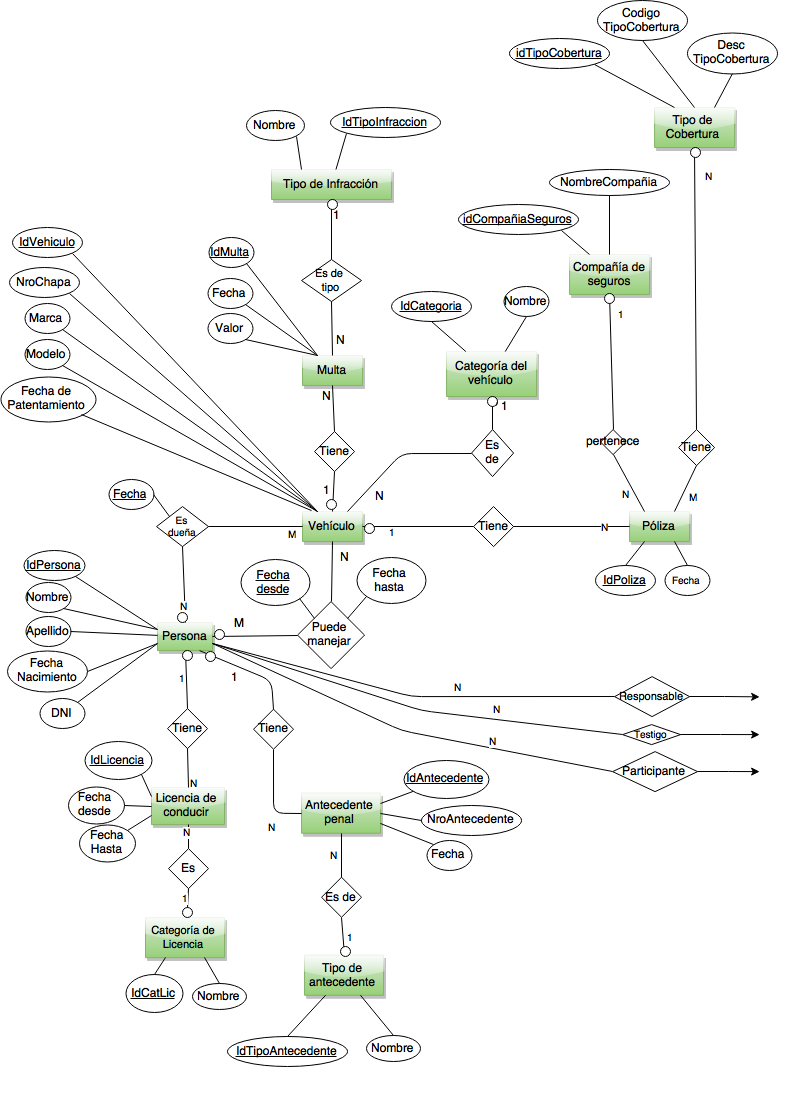
\includegraphics[width=1\textwidth]{./images/DER_1.png}
\end{figure}

\begin{figure}[h!]
  \centering
  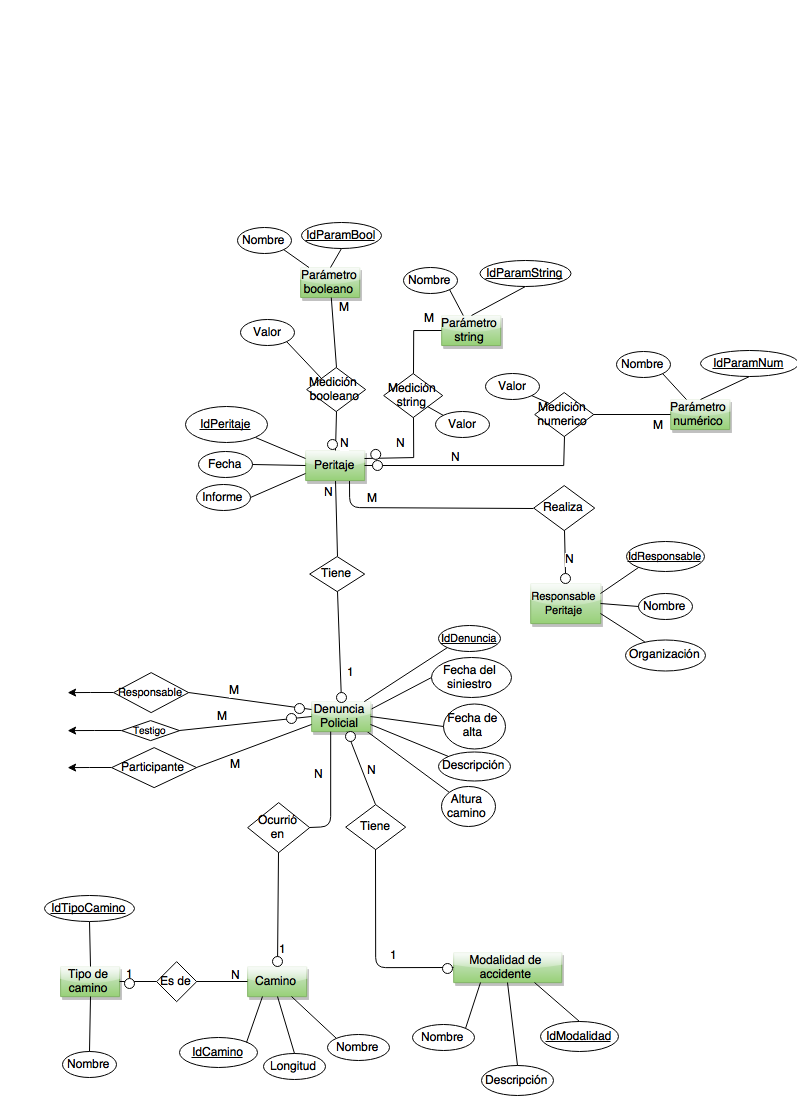
\includegraphics[width=1\textwidth]{./images/DER_2.png}
\end{figure}

\section{Modelo Relacional}
A continuación documentamos el pasaje del \textbf{DER} anteriormente expuesto al \textbf{MR} que luego será el que represente las tablas físicas en nuestra base de datos. Primero se anotan las tuplas que representan cada tabla y sus columnas, y luego, de ser necesario, las \textit{Restricciones Adicionales} (RA):\\
\\
\tuple{ParametroBooleano}{\pk{idParamBool}, Nombre}
\ra{\attr{ParametroBooleano.Nombre} no puede ser nulo.}
\\
\tuple{ParametroString}{\pk{idParamString}, Nombre}
\ra{\attr{ParametroString.Nombre} no puede ser nulo.}
\\
\tuple{ParametroNumerico}{\pk{idParamNum}, Nombre}
\ra{\attr{ParametroNumerico.Nombre} no puede ser nulo.}
\\
\tuple{MedicionBooleano}{\pk{idParamBool}, \pk{idPeritaje}, Valor}
\ra{\attr{MedicionBooleano.Valor} no puede ser nulo.}
\\
\tuple{MedicionString}{\pk{idParamString}, \pk{idPeritaje}, Valor}
\ra{\attr{MedicionString.Valor} no puede ser nulo.}
\\
\tuple{MedicionNumerico}{\pk{idParamNum}, \pk{idPeritaje}, Valor}
\ra{\attr{MedicionNumerico.Valor} no puede ser nulo.}
\\
\tuple{Peritaje}{\pk{idPeritaje}, Fecha, Informe, \fk{idDenuncia}}
\ra{\attr{Peritaje.Fecha} debe ser posterior a \attr{Denuncia.Fecha}, con \attr{Denuncia.idDenuncia} = \attr{Peritaje.idDenuncia}.}
\ra{\attr{Peritaje.Fecha} debe ser anterior o igual al día de hoy.}
\\
\tuple{RespRealizaPeritaje}{\pk{idResponsable}, \pk{idPeritaje}}
\\
\tuple{ResponsablePeritaje}{\pk{idResponsable}, Nombre, Organizacion}
\ra{\attr{ResponsablePeritaje.Nombre} no puede ser nulo.}
\ra{\attr{ResponsablePeritaje.Organizacion} no puede ser nulo.}
\\
\tuple{DenunciaPolicial}{\pk{idDenuncia}, FechaDelSiniestro, FechaDeAlta, Descripcion, AlturaCamino, \fk{idCamino}, \fk{idModalidad}}
\ra{\attr{DenunciaPolicial.FechaDelSiniestro} no puede ser nulo.}
\ra{\attr{DenunciaPolicial.FechaDelSiniestro} debe ser igual o anterior a \attr{DenunciaPolicial.FechaDeAlta}.}
\ra{\attr{DenunciaPolicial.FechaDeAlta} no puede ser nulo.}
\ra{\attr{DenunciaPolicial.Descripcion} no puede ser nulo.}
\ra{\attr{DenunciaPolicial.AlturaCamino} no puede ser nulo.}
\ra{\attr{DenunciaPolicial.AlturaCamino} no puede ser negativa.}
\ra{\attr{DenunciaPolicial.idCamino} no puede ser nulo.}
\ra{\attr{DenunciaPolicial.idModalidad} no puede ser nulo.}
\\
\tuple{ModalidadDeAccidente}{\pk{idModalidad}, Nombre, Descripción}
\ra{\attr{ModalidadDeAccidente.Nombre} no puede ser nulo.}
\ra{\attr{ModalidadDeAccidente.Descripcion} no puede ser nulo.}
\\
\tuple{Camino}{\pk{idCamino}, Longitud, Nombre, \fk{idTipoCamino}}
\ra{\attr{Camino.Longitud} no puede ser nulo.}
\ra{\attr{Camino.Longitud} no puede ser negativa.}
\ra{\attr{Camino.Nombre} no puede ser nulo.}
\ra{\attr{Camino.idTipoCamino} no puede ser nulo.}
\\
\tuple{TipoDeCamino}{\pk{idTipoCamino}, Nombre}
\ra{\attr{TipoDeCamino.Nombre} no puede ser nulo.}
\\
\tuple{Persona}{\pk{idPersona}, Nombre, Apellido, FechaDeNacimiento, DNI}
\ra{\attr{Persona.Nombre} no puede ser nulo.}
\ra{\attr{Persona.Apellido} no puede ser nulo.}
\ra{\attr{Persona.FechaDeNacimiento} no puede ser nulo.}
\ra{\attr{Persona.FechaDeNacimiento} debe ser anterior o igual al día de hoy.}
\ra{\attr{Persona.DNI} no puede ser nulo.}
\ra{\attr{Persona.DNI} no puede ser negativo.}
\\
\tuple{Responsable}{\pk{idDenuncia}, \pk{idPersona}}
\\
\tuple{Testigo}{\pk{idDenuncia}, \pk{idPersona}}
\\
\tuple{Participante}{\pk{idDenuncia}, \pk{idPersona}}
\\
\tuple{AntecedentePenal}{\pk{idAntecedente}, NroAntecedente, Fecha, \fk{idPersona}, \fk{idTipoAntecedente}}
\ra{\attr{AntecedentePenal.NroAntecedente} no puede ser nulo.}
\ra{\attr{AntecedentePenal.NroAntecedente} no puede ser negativo.}
\ra{\attr{AntecedentePenal.Fecha} no puede ser nulo.}
\ra{\attr{AntecedentePenal.Fecha} debe ser anterior o igual al día de hoy.}
\ra{\attr{AntecedentePenal.idPersona} no puede ser nulo.}
\ra{\attr{AntecedentePenal.idTipoAntecedente} no puede ser nulo.}
\nota{Ver aclaración número 2 sobre \attr{idAntecedente} y \attr{NroAntecedente}.}
\\
\tuple{TipoDeAntecedente}{\pk{idTipoAntecedente}, Nombre}
\ra{\attr{TipoDeAntecedente.Nombre} no puede ser nulo.}
\\
\tuple{CategoriaDeLicencia}{\pk{idCatLic}, Nombre}
\ra{\attr{CategoriaDeLicencia.Nombre} no puede ser nulo.}
\\
\tuple{LicenciaDeConducir}{\pk{idLicencia}, FechaDesde, FechaHasta, \fk{idPersona}, \fk{idCatLic}}
\ra{\attr{LicenciaDeConducir.FechaDesde} no puede ser nula.}
\ra{\attr{LicenciaDeConducir.FechaHasta} no puede ser nula.}
\ra{\attr{LicenciaDeConducir.FechaDesde} debe ser anterior a \attr{LicenciaDeConducir.FechaHasta}. Esto lo implementamos usando \textbf{triggers}.}
\ra{\attr{LicenciaDeConducir.idPersona} no puede ser nulo.}
\ra{\attr{LicenciaDeConducir.idCatLic} no puede ser nulo.}
\ra{Para un mismo \attr{LicenciaDeConducir.idPersona}, los rangos de Fecha de Licencia (FechaDesde~FechaHasta) son excluyentes. Es decir, una persona dada puede tener una única licencia vigente.}
\\
\tuple{Vehiculo}{\pk{idVehiculo}, NroChapa, Marca, Modelo, FechaDePatentamiento, \fk{idCategoria}}
\ra{\attr{Vehiculo.NroChapa} no puede ser nulo.}
\ra{\attr{Vehiculo.NroChapa} debe respetar el formato ``LLL/NNN'' con `L' cualquier letra mayúscula y `N` cualquier número del 0 al 9.}
\ra{\attr{Vehiculo.Marca} no puede ser nulo.}
\ra{\attr{Vehiculo.Modelo} no puede ser nulo.}
\ra{\attr{Vehiculo.FechaDePatentamiento} no puede ser nulo.}
\ra{\attr{Vehiculo.FechaDePatentamiento} debe ser anterior o igual al día de hoy.}
\ra{\attr{Vehiculo.idCategoria} no puede ser nulo.}
\\
\tuple{PersonaDuenaVehiculo}{\pk{idVehiculo}, \pk{idPersona}, \pk{Fecha}}
\ra{\attr{PersonaDuenaVehiculo.Fecha} no puede ser nulo.}
\nota{Ver aclaración número 8 sobre \attr{FechaHasta}.}
\\
\tuple{PersonaPuedeManejarVehiculo}{\pk{idVehiculo}, \pk{idPersona}, \pk{FechaDesde}, FechaHasta}
\ra{\attr{PersonaPuedeManejarVehiculo.FechaDesde} no puede ser nulo.}
\ra{\attr{PersonaPuedeManejarVehiculo.FechaHasta} no puede ser nulo.}
\ra{Una persona no puede tener una cédula azul para un vehículo del cual es dueña. Esto lo implementamos usando \textbf{triggers}.}
\ra{\attr{PersonaPuedeManejarVehiculo.FechaDesde} debe ser menor a \attr{PersonaPuedeManejarVehiculo.FechaHasta}}
\\
\tuple{CategoriaDelVehiculo}{\pk{idCategoria}, Nombre}
\ra{\attr{CategoriaDelVehiculo.Nombre} no puede ser nulo.}
\\
\tuple{Multa}{\pk{idMulta}, Fecha, Valor, \fk{idTipoInfraccion}, \fk{idVehiculo}}
\ra{\attr{Multa.Fecha} no puede ser nula.}
\ra{\attr{Multa.Fecha} debe ser anterior o igual al día de hoy.}
\ra{\attr{Multa.Valor} no puede ser nulo.}
\ra{\attr{Multa.Valor} no puede ser negativo.}
\ra{\attr{Multa.idTipoInfraccion} no puede ser nulo.}
\ra{\attr{Multa.idVehiculo} no puede ser nulo.}
\nota{La moneda representa pesos Argentinos.}
\\
\tuple{TipoDeInfraccion}{\pk{idTipoInfraccion}, Nombre}
\ra{\attr{TipoDeInfraccion.Nombre} no puede ser nulo.}
\\
\tuple{Poliza}{\pk{idPoliza}, Fecha, \fk{idVehiculo}, \fk{idCompaniaSeguros}}
\ra{\attr{Poliza.Fecha} no puede ser nula.}
\ra{\attr{Poliza.Fecha} debe ser posterior o igual al día de hoy.}
\ra{\attr{Poliza.idVehiculo} no puede ser nulo.}
\ra{\attr{Poliza.idCompaniaSeguros} no puede ser nulo.}
\\
\tuple{CompaniaDeSeguros}{\pk{idCompaniaSeguros}, NombreCompania}
\ra{\attr{idCompaniaSeguros.NombreCompania} no puede ser nulo.}
\\
\tuple{TipoDeCobertura}{\pk{idTipoCobertura}, CodigoTipoCobertura, DescTipoCobertura}
\ra{\attr{TipoDeCobertura.CodigoTipoCobertura} no puede ser nulo.}
\ra{\attr{TipoDeCobertura.CodigoTipoCobertura} no puede ser negativo.}
\ra{\attr{TipoDeCobertura.DescTipoCobertura} no puede ser nulo.}
\\
\tuple{PolizaTieneTipoDeCobertura}{\pk{idPoliza}, \pk{idTipoCobertura}}

\subsection{Otras resticciones adicionales}
\hspace{-0.5cm}\ra{\attr{Poliza.Fecha} debe ser posterior a \attr{Vehiculo.FechaPatentamiento} para todas las pólizas de un vehículo dado.}
\ra{\attr{DenunciaPolicial.FechaDelSiniestro} debe ser posterior a \attr{Vehiculo.FechaPatentamiento} para todas las denuncias en las que está involucrado un vehículo dado.}

\subsection{Equivalencias de nombres de tablas MR $\leftrightarrow$ DER}
En esta sección aclararemos el mapeo entre las tablas/tuplas del Modelo Relacional expuesto y las entidades e interrelaciones mostradas en el Diagrama Entidad-Relación, dado que por la naturaleza de la convención de lectura del mismo, al pasar a MR, algunas tablas intermedias quedaban con nombres poco descriptivos. Las equivalencias son:
\begin{itemize}
	\item ``RespRealizaPeritaje'' es ``Realiza'' de ``ResponsablePeritaje'' a ``Peritaje''
	\item ``PersonaDuenaVehiculo'' es ``EsDuena'' de ``Persona'' a ``Vehiculo''
	\item ``PolizaTieneTipoDeCobertura'' es ``Tiene'' de ``Poliza'' a ``TipoDeCobertura''
\end{itemize}

\subsection{Aclaraciones varias}
\begin{enumerate}
	\item La longitud del camino está expresada en kilómetros.
	\item En la parte de \attr{AntecedentePenal}, decidimos modelar nuestro id interno como \attr{idAntecedente}, siendo el identificador externo (propio del antecedente en el sistema de un tercero) un número distinto.
	\item La duración de las poliza de seguro es de 1 año a partir de la fecha de inicio.
	\item El informe del peritaje es un texto corto (hasta 400 caracteres).
	\item A pesar de que en el mundo real puede haber vehículos sin patente(no patentados aun), en este modelo no se incluyen esos casos para simplificar el mismo (sino requeriría identificar vehículos por número de motor, chasis, etc).
	\item Se considera que un vehiculo puede tener varias polizas.
	\item \attr{PersonaDuenaVehiculo} no tiene un campo \attr{FechaHasta} porque hasta que no lo vende es dueña del mismo.
	\item Una Póliza tiene una fecha, una compañia de seguro. Los tipos de cobertura de una poliza pueden ser varios por poliza. Por ejemplo, una poliza puede tener cobertura Contra Terceros, Incendio, Daño por Granizo, etc. Cada uno de estos es un tipo de cobertura y puede haber una poliza con varios de ellos y cada uno pertenecer a muchas polizas distintas. Por eso la relacion es N-M.
\end{enumerate}

\end{document}
%\section{Sección, título grande}
%\\
%\textcolor{white}{Sarasa engañadora de formato, jua jua}
%Esto es texto. Con doble barra invertida es el enter.
%\\
%\\
%\textit{De acá en adelante, todo lo que se explica como "para hacer x se usa y", implica que antes de y va una barra invertida}
%\\
%\\
%Con \textbf{textbf\{\}} se escribe en negrita.
%\\
%\\
%\section{Bullet \& Numbering}
%Para hacer items se usa \textbf{begin\{itemize\}} y \textbf{end\{itemize\}}, por ejemplo:
%\begin{itemize}
%	\item Esto es un ítem.
%	\item Esto es otro.
%\end{itemize}
%Con \textbf{item} se hace cada uno de los ítems. Si cambiás \textbf{itemize} por \textbf{enumerate} te lo hace enumerado. Por ejemplo:
%\begin{enumerate}
%	\item Acá está el primero.
%	\item Acá el segundo.
%\end{enumerate}
%\\
%Y así.
%\\
%\\
%\section{Tablas}
%También tenemos las tablas, que son un poco más rebuscadas. Se usa \textbf{begin\{tabular\}\{cols\}} y en cols ponemos c si queremos una columna centrada, l y r
%para otro tipo de justificación. Si las c las separás con espacios, se hacen columnas sin división. Si ponés un pipe es con una línea divisoria, dos pipes con
%dos líneas, y así. Se termina con \textbf{end\{tabular\}}. Para separar entre elementos de fila/columna se usa un ampersand (\&, y es necesario para separar
%elementos entre filas y columnas, no solo entre filas) y para cambiar de fila \textbf{SIN} linea divisoria, un \textbf{newline} ya que el doble barra invertida
%te hace un enter dentro de la celda. Con línea divisoria es reemplazando \textbf{newline} por \textbf{hline}.
%\\
%\\
%Más datos en el principio de este tex. Un ejemplo:
%\\
%\\
%\begin{tabular}{| c| c|}\hline
%    Celda 1 & Celda 2 &\hline
%    Celda 3 & Celda 4 &\hline
%\end{tabular}
%\\
%\\
%\section{Verbatim}
%\begin{verbatim}
%Esto es verbatim. Es un entorno que no le da ni 5 de pelota al formato de latex.
%Por eso mismo hay que tener cuidado con no irse de la hoja o similar.
%Sirve por ejemplo, para pseudocódigo:
%
%if (se cumple sarasa){
%    ejecuto cosito1;
%    ejecuto cosito2:
%}else{
%    ejecuto cosito3:
%}
%\end{verbatim}
%
%
%\end{document}